\section{Introduction}
\subsection{Model  Optimization with NeuronUnit}
Some neural properties can’t be easily measured in experiments. These unknown properties hamper modeling accuracy and require parameter fitting. For example, a common approach for approximating unknown ion channel densities is to ‘optimize’ the governing equations to match known waveforms. The process of optimization involves what is known as an ‘inverse’ problem where we efficiently and sparsely search for the ‘optimal’ value of an parameter that satisfies the system of equations. Computational optimization techniques are generally specific to a particular type of problem rather than being generalized. However, several notable algorithms have solved a wide range of problems including non-dominated sort 2 (NSGA2) and stochastic gradient descent (SGD). The popularity of these two algorithms relies on the ability to avoid falsely reporting a local minimum as the most optimal solution. However, of SGD and NSGA2, only NSGA2 is a natural choice for tackling multi-objective optimization problems. Default implementations of SGD are not able to utilize the principle of non-domination as an optimization strategy.\newline
\newline
There is a great diversity of real biological neurons, all of which differ substantially in their electrical behavior. There are a few different classes of general purpose neuronal models, that can reproduce these different types of electrical behaviours, given appropriate parameterizations of the models.\newline
\newline
An exisiting class of neuron model type, called The Izhikevich model was published with parameter sets believed to make the model outputs accurately align with a variety of real biological cell outputs. However since publication much very specific electro physiological recordings have accumulated, that in someways undermine model/experiment agreement. However it is now possible to constrain the Izhikevich model and find new parameterizations that more allow us to more accurately reproduce more recently published experimental data.\newline
\newline
NeuronUnit easily converts a quantitative measure of model/data agreement into a useful error signal. A very natural application of this signal is to guide the process of optimization. We have used Neuronunit to guide optimization by taking a flexible model type such as a generalized linear integrate and fire model or the Izhikevich model and constraining the model against relevant experimental data. As an example, NSGA2 was used to optimize models in conjunction with data driven tests based on pooled data from NeuroElectro.org. A variety of compact and fast single compartment models were used to explore model optimization. Figure 4 demonstrates test error at the beginning of the optimization process for models with randomly sampled parameters and the smaller error following optimization. Figure 5 shows the evolution of the error during the optimization process. \newline
\newline
Optimized neuron models may vary from their neuron counterparts for several reasons. Table 3 shows an example where optimizing the model with respect to the rheobase test comes into conflict with minimizing with respect to input resistance. The solution to the optimization problem consists of two sets of model parameters, which can resolve this conflict differently. Examining the experimental data that these tests were derived from suddenly becomes important. By examining the data, we can see if the rheobase currents and the distributions of input resistance are bi-modal and uniformly distributed. If the data is treated as uni-modal, and the uni-modal mean is used to optimize then the model, then the model is not able to satisfy both constraints simultaneously. In this case, the measurements don’t correspond to neuron data, and the model can’t produce the artificial behavior. When comparing complex data and simple models we find that solutions are better represented using a combination of two optimization solutions.\newline
\newline
Another potential issue to consider when evaluating the scientific merit of a model is that neurons may have different behaviors under different stimulation paradigms. It might be appropriate to compare modeled behavior against measurements specific to each of two or more distinct modes. In this case, when optimizing single cell models, it’s appropriate to accept a solution set, rather than a single solution. For example, the cerebellar Purkinje cell is sensitive to intricately patterned dendrite input current combinations. Depending on a cell’s recent history of synaptic stimulation, a Purkinje cell may toggle between coincidence detection and integration modes (Ratté, Hong, De Schutter, \& Prescott, 2013).\newline
\newline
\Section{Ecosystem of Modelling Resources}
The NEURON simulator is a software suite that wraps powerful and fast ordinary differential equation solvers based in the C programming language inside a mixed compiled/interpreted environment targeted at research scientists. NEURON is somewhat analogous to older, analog circuit simulators; however, rather than describing complex resistor-capacitor circuits, NEURON instead solves equations for the time varying membrane potential of multi-compartment models.\newline
\newline
These multi-compartmental models are based on cables of varying diameters and lengths that represent the morphology of neurons, where these cables support ionic currents in the membranes. These neuronal models can be coupled together into a network, where the electrical state of one neuron has an impact on the state of coupled neurons through synaptic currents. Specifying the system of differential equations representing these neuronal morphologies, ion channels, and synaptic connections is complicated, but NEURON makes multi-compartment neuron simulation efficient, convenient, and achievable. Models expressed in NEURON code are procedural in nature, and the code consists of low-level implementation details. Procedural descriptions of models are difficult to extend and re-use, leading to a need for a declarative model description language. NeuroML has been tasked with describing these with complex network models.\newline
\newline
Through jNeuroML, the NeuroML project also provides a simple code interface for generating complex simulator code, so that NeuroML models are readily exchanged between different types of simulators. Model interchange permits cross examination of results as a they vary across simulators, and this interchange promotes the movement of models between languages preferred by different modeling communities, reconciling and unifying their models. Because NeuroML is extensible and component based, it incentivizes a “plug-in” environment for including pre-existing model components in models in a different large-scale context.


\Subsection{Significance}
Beyond experimental error, it is common to observe large variations in measurements of a single electrophysiological entity from neurons of the same classification. As an example, consider that measurements of neuron membrane input resistance may be different when recorded from different samples of the same neuron type. This variation is an essential consideration when evaluating the scientific merit of a computational model of a neuron-type. In this work, we propose to perform a large-scale analysis of model against data agreement and model against model agreement to expose the variation in biophysically realistic neuron models and cortical data. By analyzing the variance in data and among models and linking the variation to specific features and mechanisms, we also will better understand the heterogeneity of experimental measurements from a particular neuron-type. Performing a meta-analysis with a large number of models will provide other insights. We will determine whether there is higher variance in modeled electrical properties versus experimental neurophysiological measurements. We will examine whether an extensive collection of cortical models behaves more similarly to each other than to the data and will answer the question: does the space of all existing single cell models accurately represent the variability in experimental data?
Similarly, variation in the behavior of cortical neuronal networks is not well quantified. Tremendous research effort has been consumed producing several high-quality, experimentally informed cortical network models. Before creating another elaborate network model, we will determine whether these pre-existing approaches lead to networks with significantly different dynamic properties. Also, we will create an infrastructure that allows scientists to quantify the similarities and differences among networks and their dynamics – both biological and in silico.\newline
\newline
Existing data sets are incomplete, consisting of a sparse sampling of cells in the rodent brain. By necessity, models are constrained using these incomplete data sets, leading to compensatory model development that synthesizes missing information. Missing data occurs at multiple levels during network construction including exact neuron to neuron wiring patterns, un-sampled morphologies, unknown synapse activation times, and unknown axon and dendrite synapse locations. Published models should not be regarded as final, but to improve models, it is vital that they are validated against newly-obtained experimental data. The proposed work will facilitate ongoing validation of biophysically realistic models. \newline
\newline

Some electrophysiology data are challenging to integrate into existing models. These include data collected from animal species that are not widely used in models such as marmoset, guinea pig, and even humans. Additionally, neuron-type data may come from a widely-used model organism, but the tissue samples may have been extracted from brain tissue in a pathological condition. In practice, open access data is not always useable, as it be derived from multiple species types and brain regions. We will obtain a better understanding of region-dependent differences and species-dependent differences in order to help researchers map models onto a standardized rodent electrophysiological phenotype space.\newline
\newline

\subsection{Innovation}
The large-scale meta-analysis described here has not been performed previously. For the first time, a large number of cortical neuron and neuronal network models are available in the standardized NeuroML format. Although the Allen Institute for Brain Science modeling project and the Blue Brain project both rigorously analyzed their single cell models, there has not been an overarching meta-analysis across different cell and network model sources. Similarly, numerous modeling efforts have employed data-driven testing in model development workflows, but all these efforts have been based on non-standard ‘in-house’ model types and execution environments. In contrast, this work proposes to expand a pre-existing standardized model testing space, NeuronUnit, that supports model validation and re-use regardless of the model source. To date various NeuronUnit tests of action potential shape, electrical properties, and single cell morphologies exist; yet these tools are not unified. Some tests of network dynamics also currently exist; however, these tests are not integrated into a unified multiscale workflow. Significantly, a unified workflow would better locate errors in network behavior which are manifest at the network level but are caused by neuron-type models. \newline
\newline

\subsection{Approach}
Many sophisticated, experimentally informed models of neurons and neuronal networks exist, yet these models are limited to the target neuron class and brain region they were designed to explain. There is a scientific and economical mandate to increase the usability of existing models and data; however, it is unknown whether models developed for a particular cortical area can be re-parameterized to model a different cortical region. A systematic and thorough comparison of neuron model behavior has not been performed, and it is unknown how differently classes of models behave relative to one another and different data. We seek to widen the range of valid model re-purposing by examining relationships across hundreds of cortical neurons, across neuron type models, and by comparing these models to experimental data.\newline
\newline
Model formats and simulation software: This project will rely on NeuroML, a community-developed format for describing multiscale models in neuroscience supported by over 40 downstream applications, including simulators, databases, and tools for analysis and 

\subsection{Further Validation of Optimized Models}
Models can continue to undergo validation checks subsequent to optimization. One way to do this is to move from a single spiking stimulus regime, to a multispiking regime, and then use different feature extraction libraries using a much larger number of features.  The higher dimensional feature space can be reduced to a low dimensional space, where it is easier to discriminate between models and data.


\section{Further Validation of Optimized Models}
Models can continue to undergo validation checks subsequent to optimization. One way to do this is to move from a single spiking stimulus regime, to a multispiking regime, and then use different feature extraction libraries using a much larger number of features. 
%Models can continue to undergo validation checks subsequent to optimization. One way to do this is to move from a single spiking stimulus regime, to a multispiking regime, and then use different feature extraction libraries using a much larger number of features. 
%The higher dimensional feature space can be reduced to a low dimensional space, where it is eaasier to discriminate between models and data.
\Section{Sensitivity Analysis and NeuronUnit Error Correlation}
Sensitivity Analysis was performed using three different combinations of model, with just one data driven suite of neuronunit tests. Sensativity analysis gives some indication of the difficulty of optimization problems.\newline
\newline
Sensitivity Analysis was able to reveal if model parameters had second order effects, that is is the model behavior dependant on not just the single parameter, but also a second intermediary parameter, and this parameter. \newline
\newline
In the Izhivitch model many of nine model parameters demonstrated significant effects.
%Agreement between the optimized.
\chapter*{Methods}
%\begin{table*}



\begin{figure}
	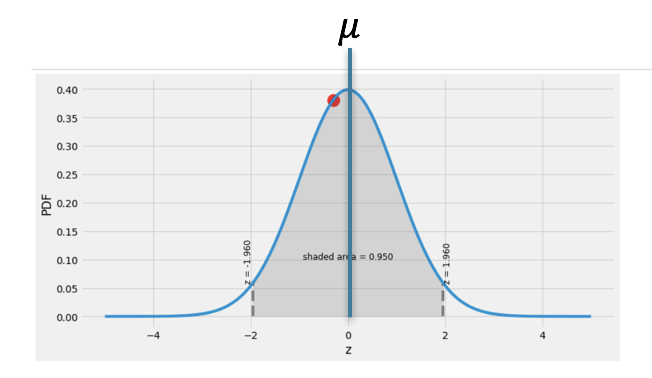
\includegraphics[width=\maxwidth{\textwidth}]{figures/normal_distribution.png}
	\caption{Error scores that came from neuronunit were based on finding a normal distribution on electro physiology measurements, and then measuring model outputs and mapping the model behavior onto a place on the experimental normal distribution. Scores that where closer to the experimental mean where deemed to be low in error.
	Z-scores obtained via NeuronUnit can be thought of as  }
	\label{figure\arabic{figurecounter}}
	
\caption{Caption}
	
\end{figure}

\begin{markdown}
| cell type   |      models      |
|----------|:-------------:|
| olfactory bulb mitral cell | layer IV pyramidal neuron |
| cerebellar purkinje cell | ca1 pyramidal cell |
| HH model score | HH Model score |
| 37.0 | [Phytochromobilin C15-Z,syn - C15-E,anti isomerization: concerted or stepwise?](https://www.researchgate.net/profile/Bo_Durbeej/publication/225093436_Phytochromobilin_C15-Zsyn_C15-Eanti_isomerization_Concerted_or_stepwise/links/0912f4fcd237e6701a000000.pdf) |
\end{markdown}

\begin{table*}
%\begin{longtable}
\centering
\resizebox{\columnwidth}{!}{
 \begin{tabular}{@{}SSSS@{}}
 	\hline 
 	olfactory bulb mitral cell & layer IV pyramidal neuron & cerebellar purkinje cell & ca1 pyramidal cell \\ 
 	\hline 
     	& HH model score &  HH Model score &  HH model score & HH model score\\ 
 	\hline 
 	& Izhikitich model score  & Izhikitich model score & Izhikitich model score& Izhikitich model score \\ 
 	\hline 

\bottomrule
\end{tabular}
}
\caption{Caption}
We optimized three classes of reduced Neural models with respect to four different experimental data types.
\end{table*}         

\chapter*{Results}
\section{PCA and tSNE}
%[width=0.5\textwidth]
%\maxwidth=0.9
%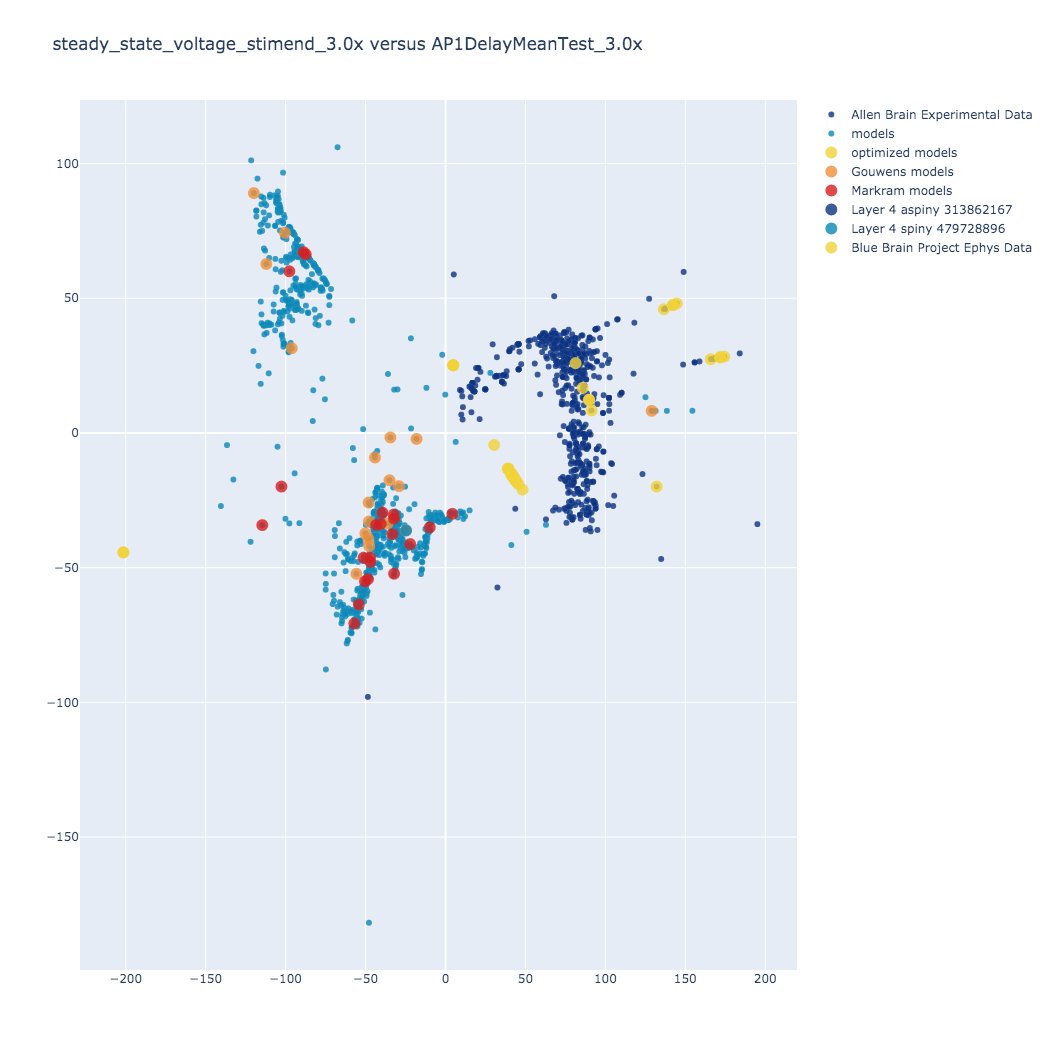
\includegraphics[width=\maxwidth{\textwidth},scale=0.5]{figures/PCA.png}

\begin{figure}

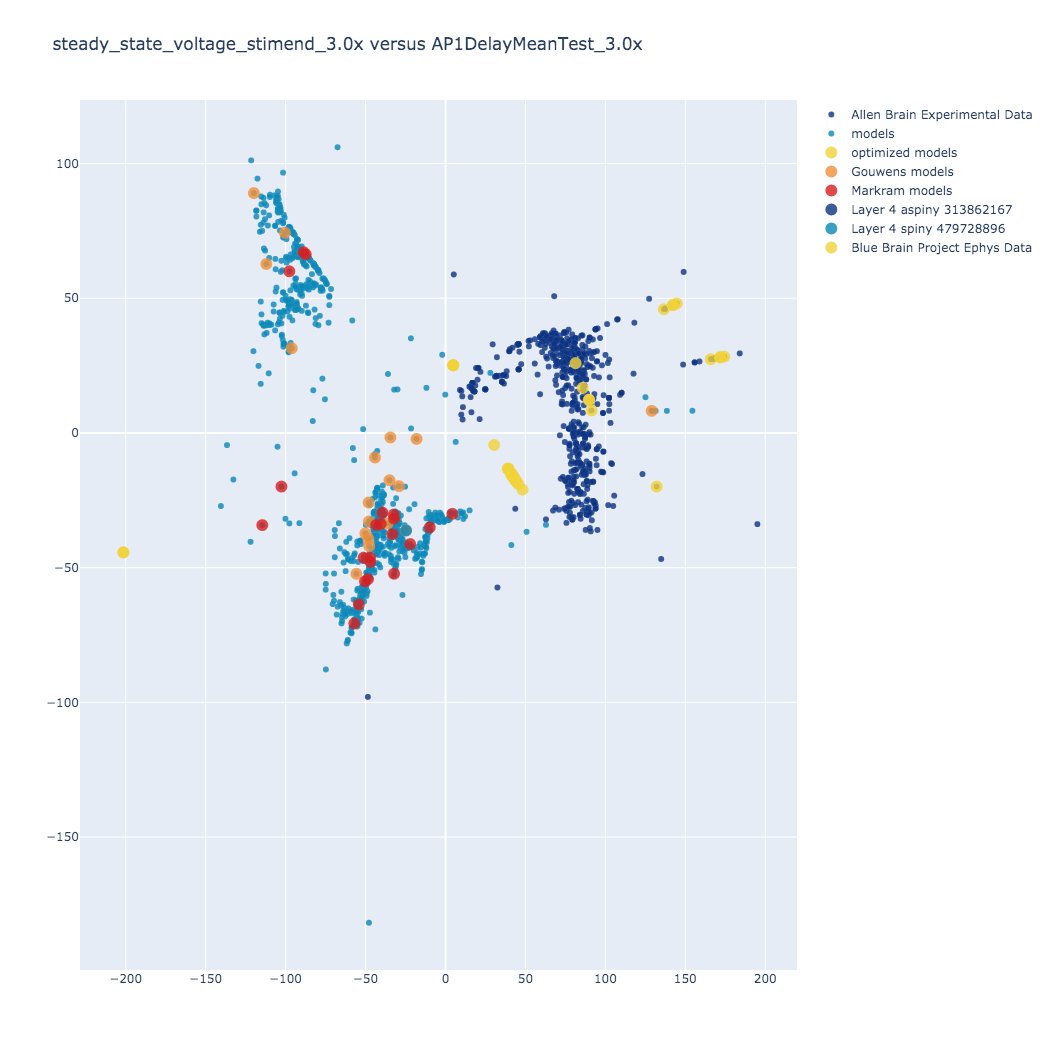
\includegraphics[width=\maxwidth{\textwidth},scale=0.5]{figures/PCA.png}
\caption{Principal Component Analysis}
\label{figure\arabic{figurecounter}}
\legend{Feature Variance distributed though-out a plane, the plane was output from applying dimension reduction to a high dimensional (552 dim) feature Space. The plane is related to two projection vectors that were  point in the directions of maximal variance in the data. Data is comprised by a collection of reduced neuronal models, and real recordings of voltage traces from neurons. Data and models are so different in this space that they are easily discriminated, and they fall into several natural clusters. Random Forests variance explained was later used to identify, dimensions that contributed the most variance.
\emph{T-Distributed Stochastic Nearest Neighbour Spatial Embedding} }

\end{figure}




I used Principle Component Analysis to examine the degree of separability between modeled neuron electrical recordings and real electrical recordings from actual neurons.\newline
\newline
If biologically realistic models were better at imitating real experimental cells, then data and models would not easily be discriminated. By plotting a 248 dimensional feature space onto a two dimensional projection space, I show that a diverse pool of data and models are readily discriminated via Random Forest Classification, a result, that leaves even some of the most optimized models lacking. The idea is that the models which are the most resistant to being correctly machine-classified as models (therefore being misclassified as data), serve as better imitations/mimics of experimental data. I also used random forest regression to investigate when experimental data inform a classifying statistical model which dimensions explain the most of the observed variance in the feature space. Variance-explained will facilitate the production of a list of improvements to make to our models in order to render models better imitations of real data.\newline
\newline
PCA, t-Distributed Stochastic Neighbor Embedding (t-SNE).
Random Forest Classification (RFC) using 248 features, and also RFC applied to just 2 features (output from PCA).
using the RFC "variance-explained" feature.

In contrast to other projects that seek to use features to seperate and classify two different categories of things that are hard to tell apart, such that humans can benefit from a fast classification of hard to discern differences in high dimensional spaces. In this project the goal is to use resistance to classification as an indicator of an optimization algorithms success, and to use machine seperation of data categories as an error signal, that directs us to precise locations of model failure. Another way of saying this, is, if a good/fair attempt at machine classification is hard, then then a different machine learning algorithm did a good job. If machine classification is very easy, the optimization algorithm did a poor job.

The application of TSNE to data was developed in a research team context on different data pertaining to ion channels, or the APs exclusively derived from models (as opposed to a combination of models and data). In the context of this project, I have used novel experimental data (pulled from the Allen Brain Portal API) and novel models (8 optimized cell models included), so I have re-applied a small amount of code from pre-established work, but I have made substantial novel contributions, by looking at different features, applying different feature engineering, applying Random Forest Classification, applying variance explained, and interpreting results. For a comparison to other pre-established work that informed this work check here

Model Optimization as a data pre-processing stage.
Before Machine Learning and analysis techniques could be applied, we needed to find optimized models. These optimized models can be understood as models that are intended to be superior mimics of real biologically derived data, as their governing equation parameters have been more rigorously constrained by a wider range of experimental data.

In order illustrate that the optimized models are better imitations of real data, four adaptive Exponential models, and four Izhikevich models each were fitted to four different classes of experimental cells see implementation in ipython notebook Notebook. These eight fitted models were subsequently fed into a Druckman feature extraction algorithm, and added as data points in a dimension reduced plot of the feature space. Many pre-existing neural models, and some Allen Brain Data where also plotted as contextual data in the same feature space.

Python, pandas sklearn, dask were all used for Model Optimization pre-processing steps, and for plotting the models in a dimension reduced feature space.

Models versus Data. Models which are resistant to being classified as models are more successful, and better representatives of data. See below.
The optimized cells were derived from a custom built parallel genetic algorithm, utilizing pre-existing python tools: DEAP and Dask. It would have been desirable to optimize the models with an algorithm from this course, such as Lasso, ridge regression, and elastic search (L1+L2)/2 regularization combined. The way I do this is to run a genetic algorithm over the data, The genetic algorithm is performing its own type of guided sparse sampling of the data.
The Druckman feature analysis protocol originates from MATLAB code associated with the analysis of Blue Brain Project Modelled cells, this feature analysis pipeline was then ported to Python by Justas Birgiolas, at a later point I made the feature analysis pipeline applicable to optimized Adaptive Exponential and Izhiketch cells. Rick Gerkin and Vergil Haynes, assisted in data cleaning preperation and TSNE application

\begin{figure}
	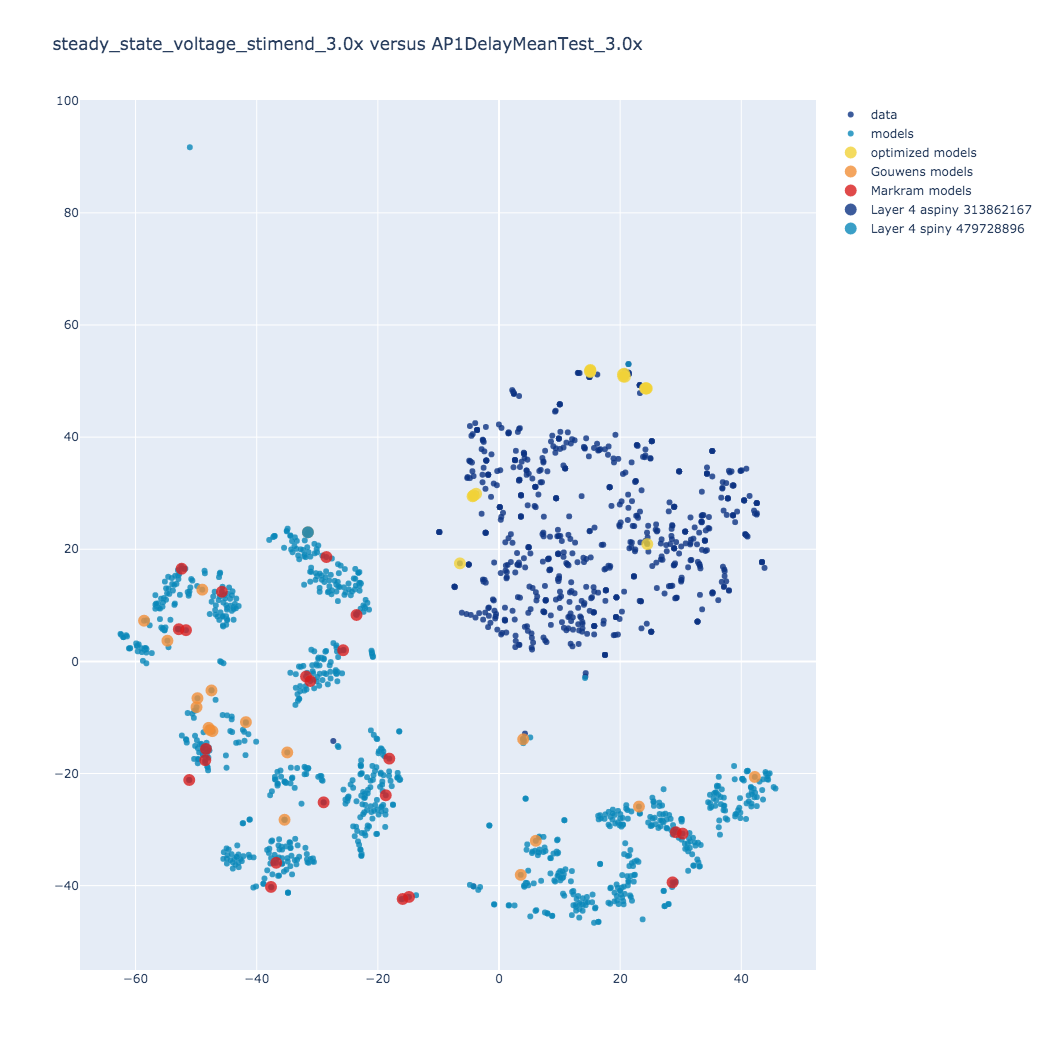
\includegraphics[width=\maxwidth{\textwidth}]{figures/TSNE.png}
	\caption{t distributed stochastic Neigherset Neighbour Spatial Embedding}
	\label{figure\arabic{figurecounter}}
\end{figure}

\begin{figure}
	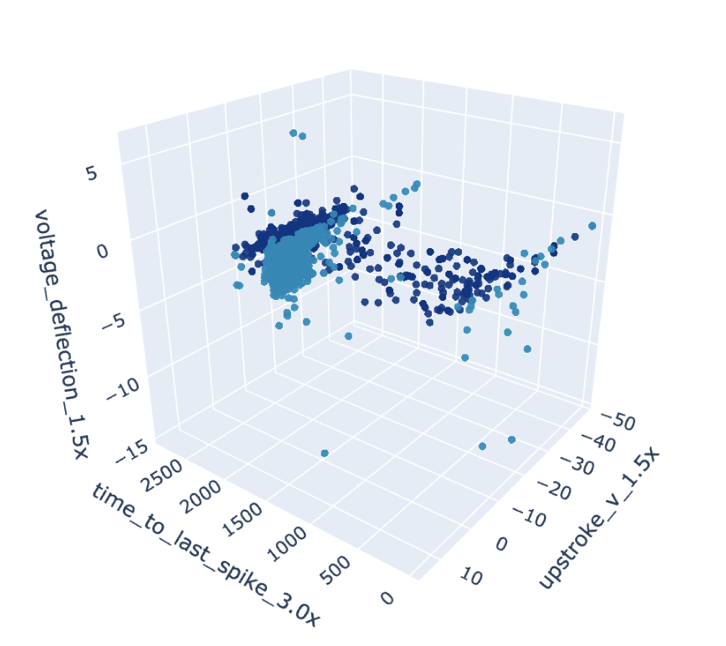
\includegraphics[width=\maxwidth{\textwidth}]{figures/directions_variance.png}
	\caption{A 3D scatter plot of the features that contributed the highest variance explained using Random Forest Classification.}
	\label{figure\arabic{figurecounter}}
\end{figure}
\begin{figure}
	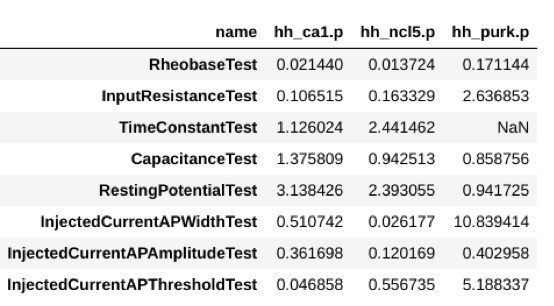
\includegraphics[width=\maxwidth{\textwidth}]{figures/results_conductanc_models.png}
	\caption{This Plot demonstrates good agreement between a simulated data and an optimised model.}
	\label{figure\arabic{figurecounter}}
\end{figure}
\begin{figure}
	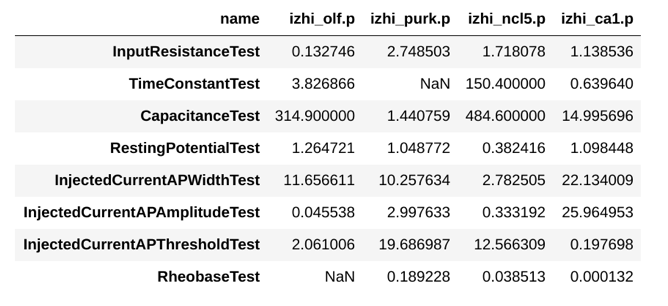
\includegraphics[width=\maxwidth{\textwidth}]{figures/results_izhi_models.png}
	\caption{t distributed stochastic Neigherset Neighbour Spatial Embedding}
	\label{figure\arabic{figurecounter}}
\end{figure}

\begin{figure}
	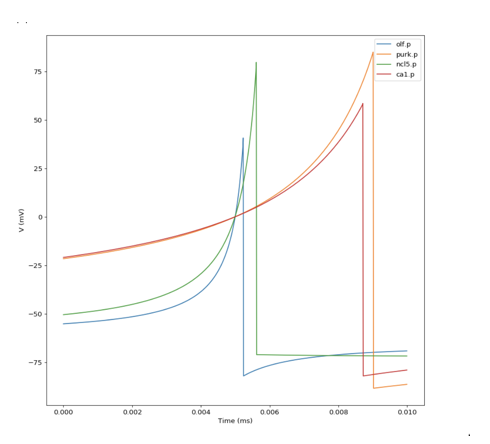
\includegraphics[width=\maxwidth{\textwidth}]{figures/results_izhi_waves.png}
	\caption{t distributed stochastic Neigherset Neighbour Spatial Embedding}
	\label{figure\arabic{figurecounter}}
\end{figure}
\begin{figure}
	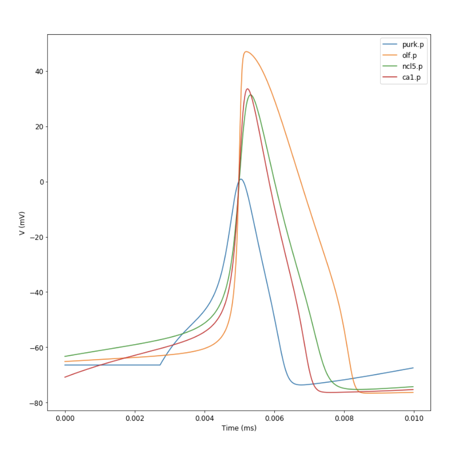
\includegraphics[width=\maxwidth{\textwidth}]{figures/results_conductance_waves.png}
	\caption{t distributed stochastic Neigherset Neighbour Spatial Embedding}
	\label{figure\arabic{figurecounter}}
\end{figure}


\Chapter*{Optimization_of_existing_models_to_align_them_with_data}
\Chapter*{Optimization_of_models_to_find_diverse_solutions_for_the_same_behaviors}        
\Chapter*{Technical_details_of_optimizer}
\Chapter*{Verification_of_the_optimizer}



%\begin{tabular}{@{}lll@{}} …
%\begin{centre} 
                               
                                        

